\section{Implementation Highlights}\label{sec:impl}

\subsection{Marks management classes}
\texttt{Course} (formerly \texttt{Module}) stores the course code and name together with two \texttt{ArrayList} collections, one of \texttt{AssessmentComponent} objects and one of \texttt{Student} objects. \texttt{AssessmentComponent} keeps four private attributes (key, label, weight and maximum mark) and exposes them through accessors, which is encapsulation in practice \cite{geeksEncapsulation}: other classes can read an assessment's weight but cannot change it by accident.

\texttt{IndividualMarksManager} does the processing. Its constructor and its three setters pass every non-null mark through a private \texttt{isValidMark()} method that accepts only the range 0--100, and throw \texttt{IllegalArgumentException} otherwise. Figure~\ref{fig:impl-code} shows the weighted calculation.

\begin{figure}[htbp]
\centering
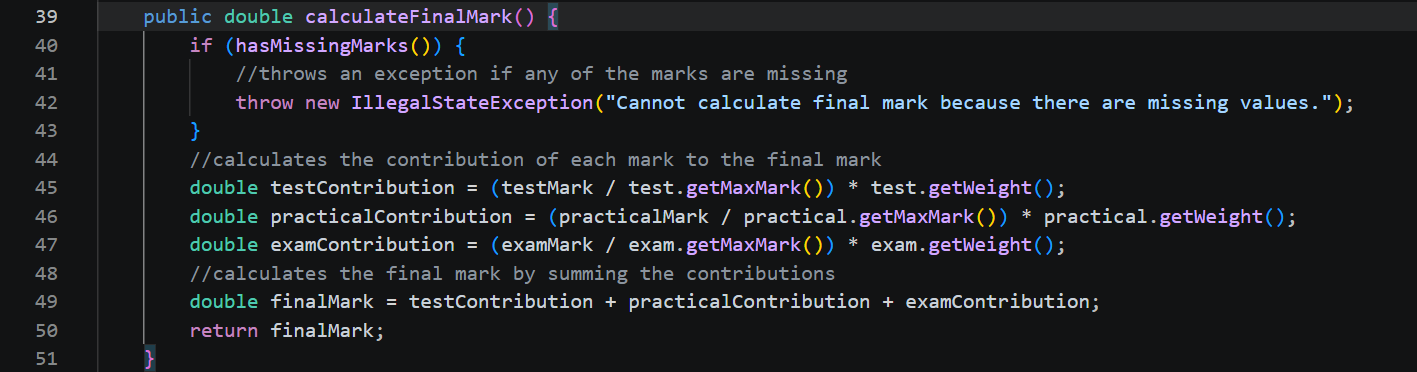
\includegraphics[width=0.92\textwidth]{Images/ch4_weighted_calculation.png}
\caption{Weighted contribution of each assessment in \texttt{IndividualMarksManager}.}
\label{fig:impl-code}
\end{figure}

\subsection{Persistence}
The \texttt{Database} class uses \texttt{java.nio.file} \cite{oracleFiles}. \texttt{saveData} builds a list of lines (a header followed by one line per student from the \texttt{StudentManager}), creates the parent folder with \texttt{Files.createDirectories} if needed, and writes the lines with \texttt{Files.write}. The course code is taken from the file name by removing the \texttt{marks.csv} suffix. Together with \texttt{loadData}, which skips blank, comment and header lines before building one \texttt{Student} per record, this provides create, read, update and delete behaviour on a plain text file. Output lines follow a fixed layout of student ID, name, assessment marks, final mark, grade and status.

Two design points are worth recording. First, \texttt{exportCSV} takes the destination \texttt{Path} as a parameter instead of prompting on the console, so any interface can call it. Second, \texttt{saveData} replaces the whole file, so saving without loading first would overwrite existing data. Course data is therefore loaded when a course is selected, before any edit is saved. The unused \texttt{importCSV} method was deleted once \texttt{importMarks} in \texttt{Lecturer} covered the same work, rather than keeping two import routes.

\subsection{Role layer and session handling}
Each role method exists in two forms. The parameterless form follows the Check-in 1 UML. The form that takes parameters and returns a \texttt{String} is what the interface calls, for example \texttt{viewClassSummary(course)} for the Head of Department. Both forms delegate to \texttt{CollectiveMarksManager} for statistics, so the maths is written once. \texttt{CourseSessionCoordinator} hands the interface the \texttt{StudentManager} and \texttt{Database} of the selected course.
